\section{Overview over the proposed pipeline}~\label{seg:ov_pip}

To overcome the two problems stated in the previous section, the following is done. Making hard decisions on merges and unmerges between superpixels is bad because of the arising contradictions where cycle constrains easily become violated but also because a hard thresholding of predictions has to be performed which takes away all the information that lies in the uncertainty of this predictions.\\
Both those issues can be overcome by predicting affinities on the edges between neighboring superpixels which can be transformed into costs and a minimum cost multicut (see section \ref{sec:multicut}) of the superpixel graph can be computed. This leverages the uncertainty of the network predictions and overcomes violated cycle constraints.\\
The second issue that arises from the irregularity of the superpixel graph can be overcome by using a graph neural network (GCNN)that predicts edge weights between superpixels by performing graph convolutions (see section \ref{sec:gcn}). However this generates the problem that there have to be regular representations for superpixels. Of course one solution would be to have two GCNNs, one for intra superpixel convolution and pooling, down to a vector representation of each superpixel and one for inter superpixel convolution using the vector representations. The problem here is the intra superpixel GCNN. Regular graph covolutions on image data makes not a lot of sense because it is not able to capture spatial information like object shapes very good. There are some proposals \cite{monti2016geometric} that introduce spatial dependent features to graph cnvolutions. However considering the power of CNNs with regular images, it makes more sense to use those in favor of GCNNs.\\
Getting superpixel representations from a CNN can be done using a embedding network that predicts pixel embeddings by minimizing a contrastive loss (see section \ref{ssec:loss_contrastive}). Still assuming, that the ground truth segmentation is a partitioning of the superpixels, it is safe to assume similar pixel embeddings in terms of the distance used in the loss for all pixels within a superpixel. Therefore one can average over all pixel embeddings within a superpixel in order to arrive at a vector representation that is used as node features in the following GCNN.\\
The described model is depicted in figure \ref{overview}.


\begin{figure}[ht!]
	\centering
	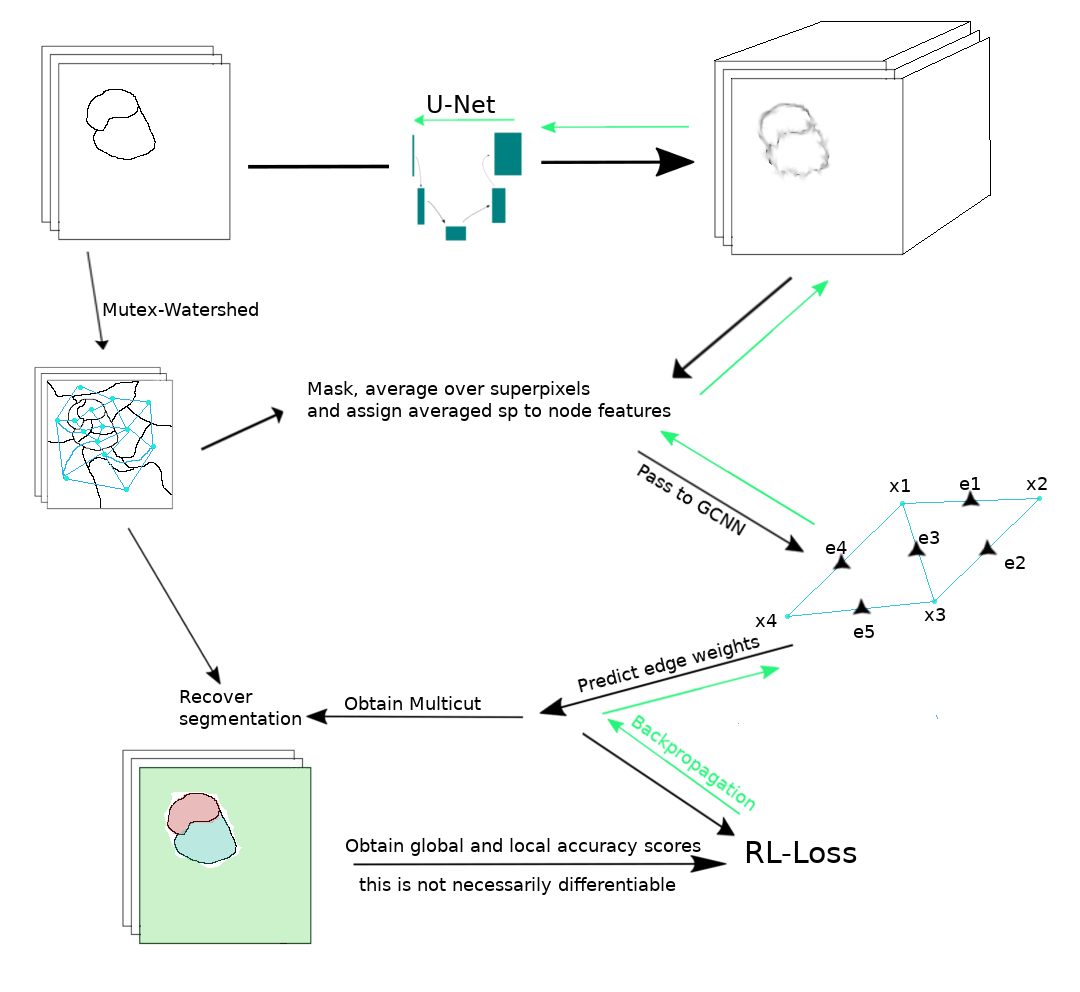
\includegraphics[width=1\textwidth]{figures/images/sketch_overall.png}
	\caption{A rough sketch of the proposed pipeline. Starting from raw data (top left), a superpixel graph is obtained with the Mutex Watershed algorithm \ref{algo:mtx_wtsd} and pixel embeddings (top right) are obtained with an embedding network. With node features computed as the average pixel embedding per superpixel a GCNN predicts logits on the edges of the superpixel graph. The logits are used to compute chances which in turn are used to compute costs based on which a min cost multicut of the superpixel graph is computed from which a segmentation is obtained. This segmentation is then evaluated and a reward is produced which is then used in the RL loss.}
	\label{overview}
\end{figure}


The following sections go into detail of every part in the sketch in figure \ref{overview}